% \textbf{Title: Bode Diagram 3}

Consider this Bode diagram of a continuous-time filter.

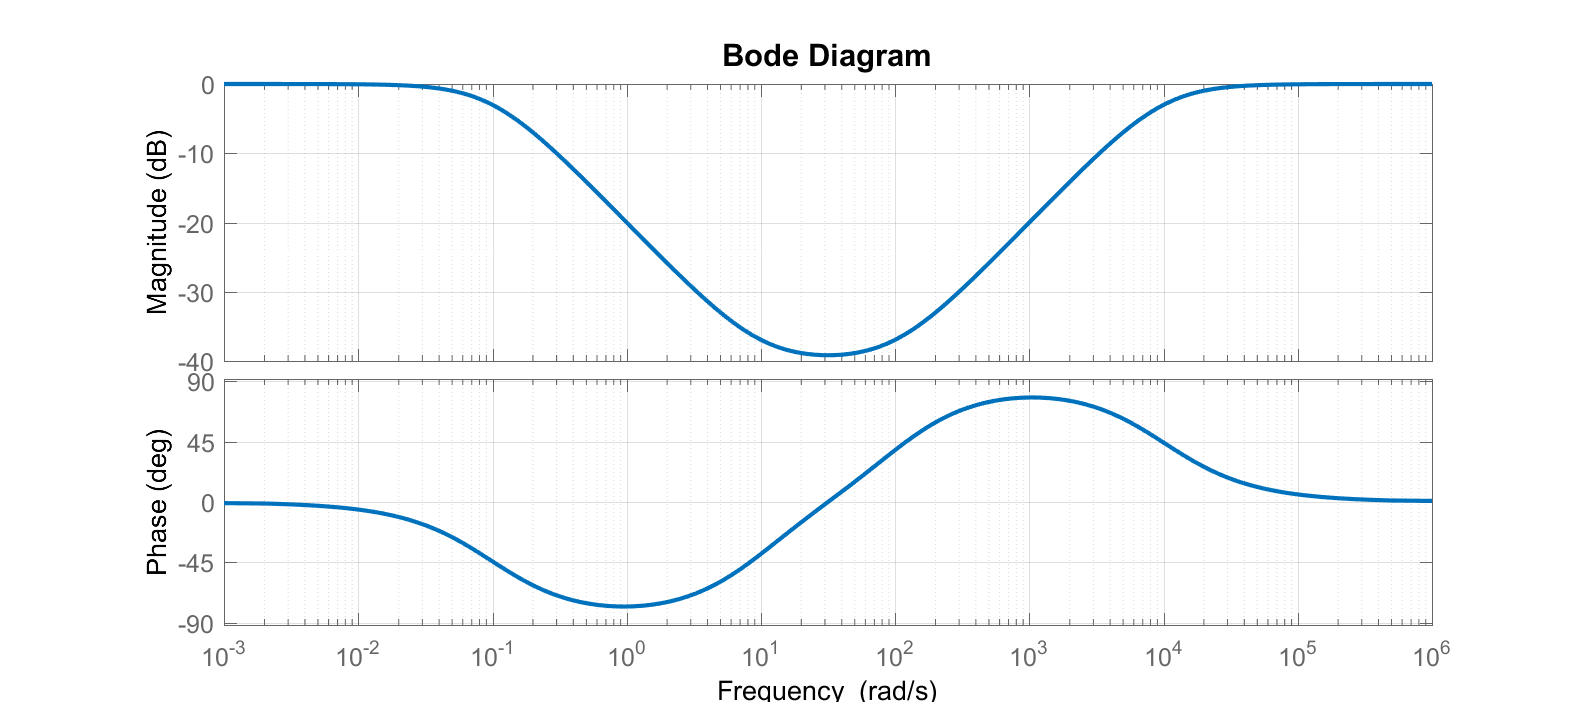
\includegraphics[width=6.07864in,height=2.69855in]{../../Images/BodeDiagramQ3.png}

If the frequency components in the pass band must be attenuated by at most \(3\ \text{dB}\) and the frequency components in the stop band must be attenuated by at least \(20\ \text{dB}\), where is the transition band?\\

a. Between the frequencies \(0.1\ \text{rad/s}\) and \(1\ \text{rad/s}\).

b. Between the frequencies \(1,000\ \text{rad/s}\) and \(10,000\ \text{rad/s}\).

c. Between the frequencies \(0.1\ \text{Hz}\) and \(1\ \text{Hz}\) as well as \(1,000\ \text{Hz}\) and \(10,000\ \text{Hz}\).

*d. Between the frequencies \(0.1\ \text{rad/s}\) and \(1\ \text{rad/s}\) as well as \(1,000\ \text{rad/s}\) and \(10,000\ \text{rad/s}\).

e. I do not know.\\
